\chapter{Introduction}\label{ch:introduction}
Filesender applications, such as the popular WeTransfer\footnote{\url{https://wetransfer.com}} or its self-hosted open source alternative FileSender project\footnote{\url{https://filesender.org}}, are a popular way to transfer large amounts of data, removing the file size restrictions of regular email.
Due to their popularity, filesender services are a privacy hotspot, too.
That is, large amounts of possibly privacy-sensitive data are uploaded to these services and a possible security breach at such a service could give adversaries access to the data of numerous users.
To improve privacy, end-to-end encryption is required for services like these.

Implementing end-to-end encryption however comes with the problem of key management.
With symmetric encryption, key management can be problematic as keys need to be shared out-of-band via a different secure channel.
The confidentiality of the transfer then is transferred to the confidentiality of this other channel.
In practice with negligent users, this often results in keys being shared unencrypted via email.
Asymmetric encryption could solve this problem, but the practicalities of properly running a dedicated public key infrastructure or alternative infrastructure (like PGP Web of trust\footnote{\url{https://en.wikipedia.org/wiki/Web_of_trust}}) for this purpose, might be even more problematic.

\section{About SURF}\label{sec:about-surf}
SURF is the Dutch organisation of collaborative educational institutions.
SURF offers ICT services to their members, among which some cloud services such as SURFfilesender, that is based on the open source FileSender project.
Via SURFfilesender, students and staff from these institutions can share large files (up to 1TB) with each other.
SURF has a high focus on security and privacy and thus does not want to process large amounts of unencrypted data with their service.

\subsection{Current end-to-end encryption in the FileSender project}\label{subsec:current-end-to-end-encryption-in-the-filesender-project}
Currently, the FileSender project does implement end-to-end encryption with symmetric encryption (via passwords and PBKDF2).
When users choose to use this option, they are asked to choose or generate a password.
This password is then used to encrypt the files in browser, before they are uploaded to the server.
When the file upload is complete, the server returns a link that can be shared with the recipient in order to download the files.
The password is not sent to the server, but is expected to be shared out-of-bands with the recipient.
When downloading the files, the recipient is required to enter the password, which is then used to decrypt the files in browser again.

This way, though SURF does facilitate the transfer of data for their users, they do not have access to the data itself.
Also, in a way, this could be considered as a form of two-factor authentication, as the files can only be retrieved with access to the download link (send via email to the user's email box) and with knowledge of the password.
This, in principle, makes the service suitable for transferring privacy-sensitive data.

\subsection{Problems with the current end-to-end encryption}\label{subsec:problems-with-the-current-end-to-end-encryption}
The current end-to-end encryption scheme works well, as long as the password has sufficient entropy and is shared securely with the recipient via a different secure channel.
However, in practice, SURF experiences this is often not the case.
Users often share the password via the same email that contains the download link.
This is problematic for multiple reasons.

\begin{enumerate}
    \item The password is sent in the same email as the download link, which means that we do not really have two-factor authentication for the download.
    \item The password is sent in plain text, which means that the password is not protected against eavesdropping.
    \item The recipient is made responsible for the secure handling of the password.
\end{enumerate}

Considering these problems, though the current end-to-end encryption scheme works good in theory, in practice it is not sufficient for SURF to be able to offer a service that is suitable for transferring privacy-sensitive data.
Given this situation, SURF is looking for a solution that allows them to provide end-to-end encryption for their users, without the need for the users to share the password out-of-band, guaranteeing this 2FA-like behaviour.

\section{Remote Document Encryption}\label{sec:remote-document-encryption}
In 2017, Verheul proposed Remote Document Encryption (RDE) as a scheme for `encrypting data for e-passport holders'~\cite{verheul2017remote}.
E-passports are passports that contain a chip implementing the ICAO 9303 standard~\cite{icao9303securitymechanisms}.
We immediately note that although only passports implement this standard, also other documents like national ID cards and drivers licenses, implement significant parts of this standard and can thus be used as well.
In the rest of this report, we will use the term e-passport, passport, or document interchangeably to refer to these documents, unless otherwise specified.
The RDE scheme is based on the idea that the e-passport can be used as a wireless HSM (Hardware Security Module), generating symmetric keys (shared secrets with some other party) that can be used for encryption.
In this terminology, we consider \textit{recipients} as the document holders, and \textit{senders} as the parties that want to send data to the recipients in an encrypted way.

\subsection{RDE scheme in short}\label{subsec:rde-scheme-in-short}
Recipients in this scheme first need to register their e-passport for usage with RDE, for which some data from the e-passport is extracted.
These are called enrollment parameters and one could consider them as the RDE public key of the e-passport.
Senders can then, based on this public key, generate a secret key that is shard between them and the e-passport, together with so-called decryption parameters.
The passport holder can use these decryption parameters, together with their e-passport to retrieve the secret key.
The decryption parameters here do not need to stay secret, as they are only used to retrieve the shared secret from the e-passport.
A very simplified version of the RDE scheme is shown in Figure~\ref{fig:rde-scheme-very-simple}.
\begin{figure}
    \centering
    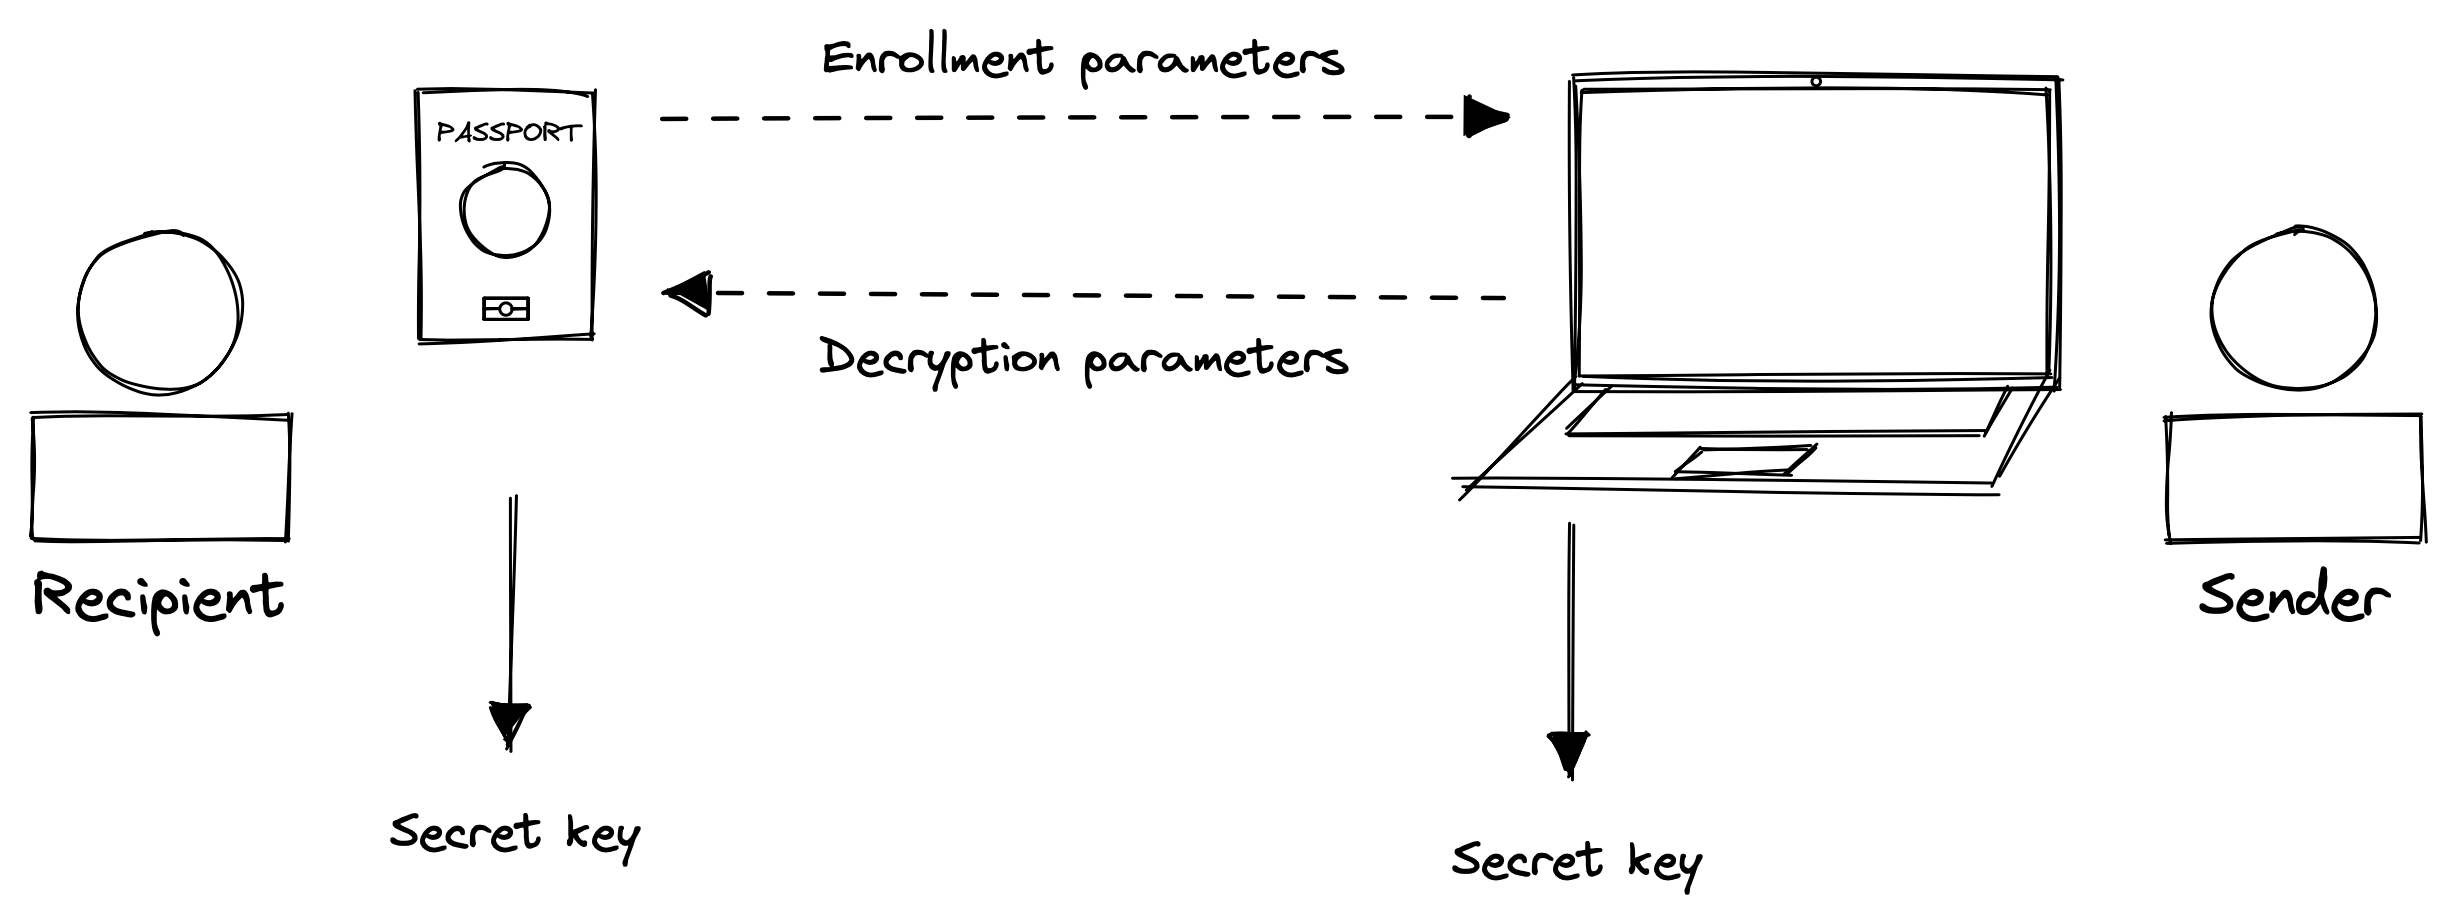
\includegraphics[width=0.8\textwidth]{imgs/RDE very simple}
    \caption{Simplified version of the RDE scheme.}
    \label{fig:rde-scheme-very-simple}
\end{figure}

\subsection{Authenticating the e-passport holder}\label{subsec:authenticating-the-e-passport-holder}
In its most basic form, the RDE scheme does not authenticate the e-passport holder.
The passport here just serves as an HSM (Hardware Security Module) that can output a key based on some input.
This already makes the scheme suitable for end-to-end encryption, as the sender and the recipient can use the key to encrypt and decrypt the data without actually having to share the key with each other.
However, the RDE scheme can be extended to also authenticate the e-passport holder using the government PKI (Public Key Infrastructure) that is used for e-passports.

In 2020, Verheul further described a secure filesender service based on RDE, where the e-passport holder is authenticated using the existing PKI for e-passports~\cite{verheul2020secure}.
During registration, additional data is extracted from the e-passport, which is used to authenticate the e-passport holder.
This includes for example the name, nationality and date of birth of the e-passport holder, but could also include other data, such as the facial image of the e-passport holder.

\section{SURFfilesender with RDE}\label{sec:surf-filesender-with-rde}
In this report, we describe how the SURFfilesender (or actually, the FileSender project) can be extended with RDE to provide end-to-end encryption for their users, without the need for the users to share the password out-of-band.
We describe an infrastructure for using RDE in applications, where we specifically focus on the SURFfilesender.
The infrastructure, however, can be used for other applications as well.

For this prototype, a number of components have been developed, which are described in the following sections.
Some components form the basis of the RDE scheme, while others are specific to the SURFfilesender application.
Especially the latter ones are not meant to be used in a production environment, but are only meant to be used as a proof-of-concept to demonstrate the feasibility of the proposed solution.
Most notably, our prototype does not implement protection against, for example, phishing attacks, denial of service attacks, or active MITM attacks on parts of the protocol that do not involve RDE itself.
We consider the challenge to implement such protections to be very much feasible, but out of scope for this report.

A proof-of-concept implementation is available at \url{TODO} and the source code is available at \url{TODO}.

\subsection{Alterations to the original secure filesender proposal}\label{subsec:alterations-to-the-rde-scheme}
Verheul already described a secure filesender service based on RDE, where the e-passport holder is authenticated using the existing PKI for e-passports~\cite{verheul2020secure}.
Though the name suggests differently, the term `filesender service' in his paper does not refer to the actual FileSender project, but to a generic filesender service.
The focus of this paper is on the SURFfilesender specifically.

Though the general outline of the RDE scheme in our report is the same, the implementation we describe in this report is notably different from the proposal in~\cite{verheul2020secure} and more closely follows the original RDE scheme as described in~\cite{verheul2017remote}.

The main reason for this is that the open source FileSender project already has end-to-end encryption implemented, which we can use as a basis for our implementation.
We thus only use the key agreement part of the scheme, and use the existing end-to-end encryption implementation of the FileSender project for the actual encryption of the files.

Moreover, we take a different approach to the authentication of the e-passport holder, because the proposal by Verheul is not compatible with SURF's way of operating.
Our more naive approach does not require any trust in SURF for authentication of users, and does not require SURF to process any sensitive data that may not be revealed to others.
This does come at the cost of less privacy for the e-passport holders, but with recent developments with Dutch e-passports, this may not be a problem anymore.

\subsection{Benefits of the proposed solution}\label{subsec:benefits-of-the-proposed-solution}
The proposed solution has a number of benefits over the current (password-based) end-to-end encryption scheme of the FileSender project.

\subsubsection{True end-to-end encryption}\label{subsubsec:true-end-to-end-encryption}
First of all, the proposed solution does not require the users to share a password out-of-band.
Instead, the encryption key is retrieved from the e-passport and never sent over a network (in unencrypted form).
Consequently, the proposed solution provides 2FA-like functionality for the download of the file: the recipient of a file transfer needs to both know the download link (that is unique and should only be sent to the recipient obviously) and be in possession of and the e-passport in order to retrieve the files.

\subsubsection{'People already have an e-passport'}\label{subsubsec:people-already-have-an-e-passport}
The aforementioned benefits, however, are not specific to the usage of RDE with e-passports.
In fact, the same benefits can be achieved by using any other HSM, such as a Yubikey, or even a smartphone.

An additional advantage of using an e-passport is that they are already widely available (`everybody has one'\footnote{
    It is a huge misconception that everyone in the world has a passport or national identity card.
    Even within the Netherlands, it is technically not mandatory to have one, only when you are somewhere in public space.
    Generally, though, and especially in Europe, it is very common to own such a document.}),
and that they are already used for authentication purposes.
For organisations like SURF and its members, this means that there are no additional costs involved in the usage of end-to-end encryption.

Another advantage is that, in contrast to using commercial HSM devices, users have an intrinsic interest in keeping their passport secure.
People are unlikely to share their passport with others or leave it somewhere unattended, as this could lead to the passport being stolen or lost and possible identity theft.
We expect people to handle their passport more securely than any commercial HSM device.
And generally, at least in the Netherlands, people are more likely to always have their identity documents with them, while commercial HSM devices or even phones might not be available at all times.

\subsubsection{Use existing governmental PKI}\label{subsubsec:use-existing-governmental-pki}
Moreover, using e-passports comes with the additional benefit that the e-passport holder can be authenticated using the existing PKI for e-passports run by governments.
Specifically for SURF, this means that SURF does not need to be responsible for the authentication of the recipient.
This is done via the government.
This is especially important as the recipients of the SURFfilesender are not necessarily affiliated with SURF itself (but with its members).
This means that SURF cannot be making claims about their identity themselves, as it does not know them directly.
